\subsection{Single Cell BES1 Model}

\begin{supplementaryfigure}[!htbp]
    \centering
    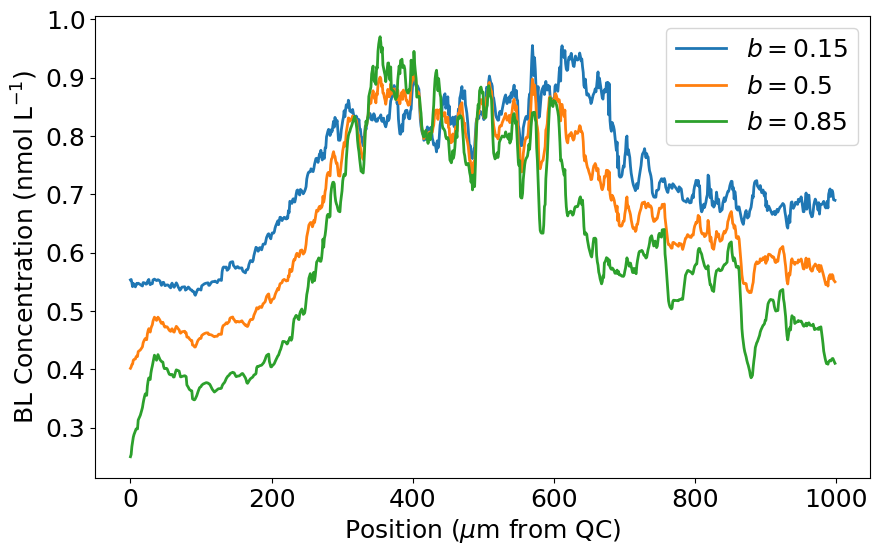
\includegraphics[width=13cm]{img/bl-bias.png}
    \caption{The BL concentration function for three different values of the bias parameter $b$. For future simulations we will use $b = 0.5$, since the BL concentration function exhibits similar qualitative behaviour for all $b$ as shown above.}
    \label{sfig:bl-bias}
\end{supplementaryfigure}

\begin{supplementaryfigure}[!htbp]
    \centering
    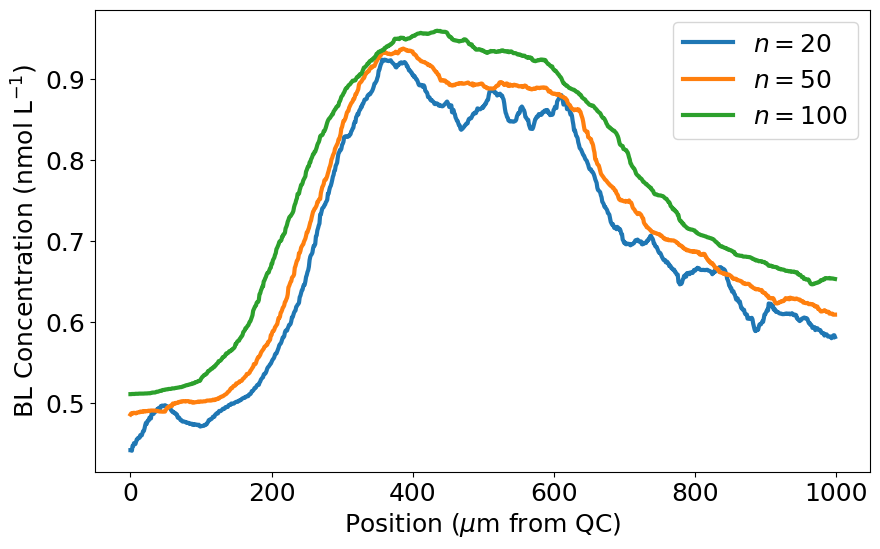
\includegraphics[width=13cm]{img/bl-average.png}
    \caption{A plot of BL concentration functions ($b = 0.5$) for three different values of the moving average period $n$. Future simulations will use $n = 50$, an admittedly arbitrary choice since the exact details of the diffusive effect we are modelling are unknown.}
    \label{sfig:bl-average}
\end{supplementaryfigure}

\begin{supplementaryfigure}
    \centering
    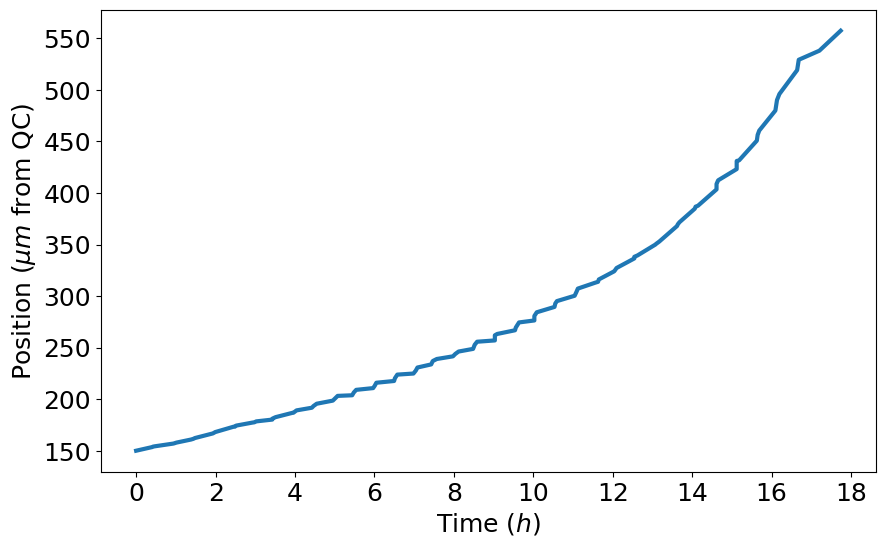
\includegraphics[width=13cm]{position-function.png}
    \caption{Plot of cell position (in $\um$) versus time (in $\h$) using cell lineage data from \cite{goh2023}. The function is scaled such that $t = 0\h$ corresponds to a position of $150\um$ above the QC.}
    \label{sfig:position-function}
\end{supplementaryfigure}

\begin{supplementaryfigure}
    \centering
    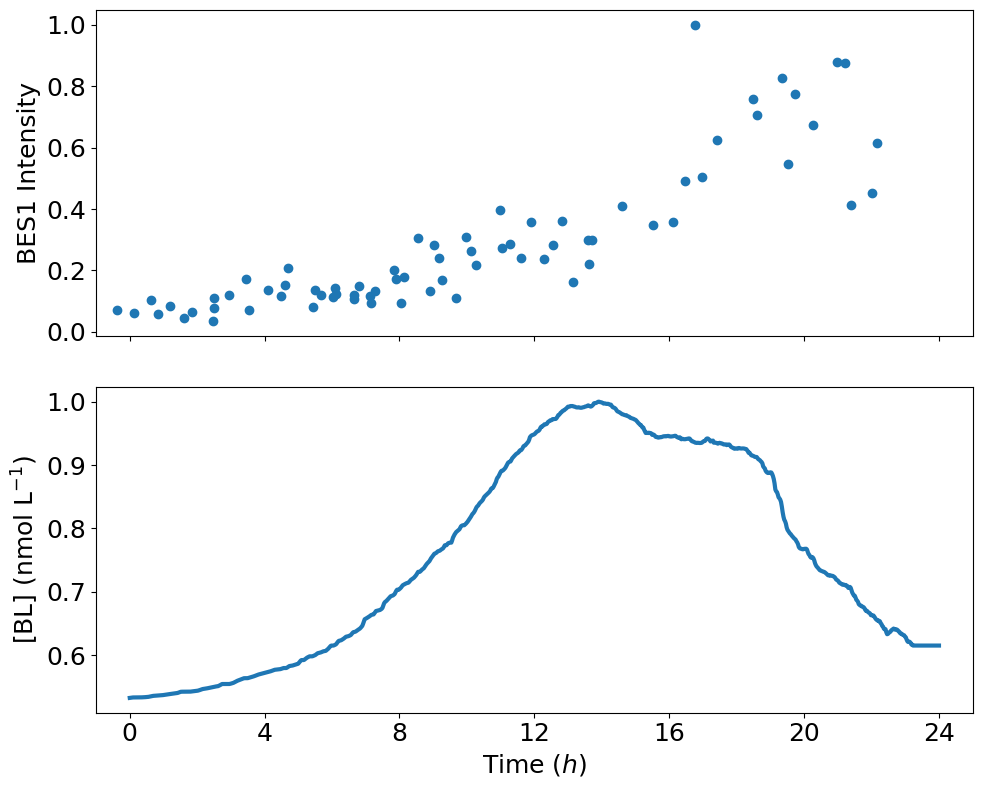
\includegraphics[width=13cm]{bes1-data.png}
    \caption{Plot of the transformed BES1 signalling data from \cite{vukasinovic2021} (left) and transformed BL concentration function (right). Since fluorescence intensity data is measured in arbitrary units, the BES1 plot was rescaled to a maximum value of $1$.}
    \label{sfig:bes1-data}
\end{supplementaryfigure}



